\documentclass[11pt]{article}
\usepackage{graphicx}
\usepackage{geometry}
\usepackage{amsmath,amssymb}
\usepackage{booktabs}
\usepackage{pifont}
\usepackage{enumitem}
\usepackage{hyperref}

\geometry{a4paper, margin=1in}
\newcommand{\CHECK}{\ding{51}}

\title{Gate Level Minimization Lecture Notes}
\author{Group 13}
\date{\today}

\begin{document}

\maketitle

\section{Introduction}
Gate-level minimization is the process of finding optimal implementations of Boolean functions using logic gates. Key aspects include:
\begin{itemize}
\item Reducing number of gates and inputs
\item Minimizing propagation delays
\item Simplifying circuit layout
\end{itemize}

\section{Karnaugh Map Method}
\subsection{Basic Principles}
\begin{itemize}
\item Visual representation of truth tables
\item Adjacent cells differ by one variable (Gray code)
\item Effective for functions with 2-5 variables
\item Two standard forms:
  \begin{itemize}
  \item Sum-of-Products (SOP)
  \item Product-of-Sums (POS)
  \end{itemize}
\end{itemize}

\begin{figure}[htbp]
\centering
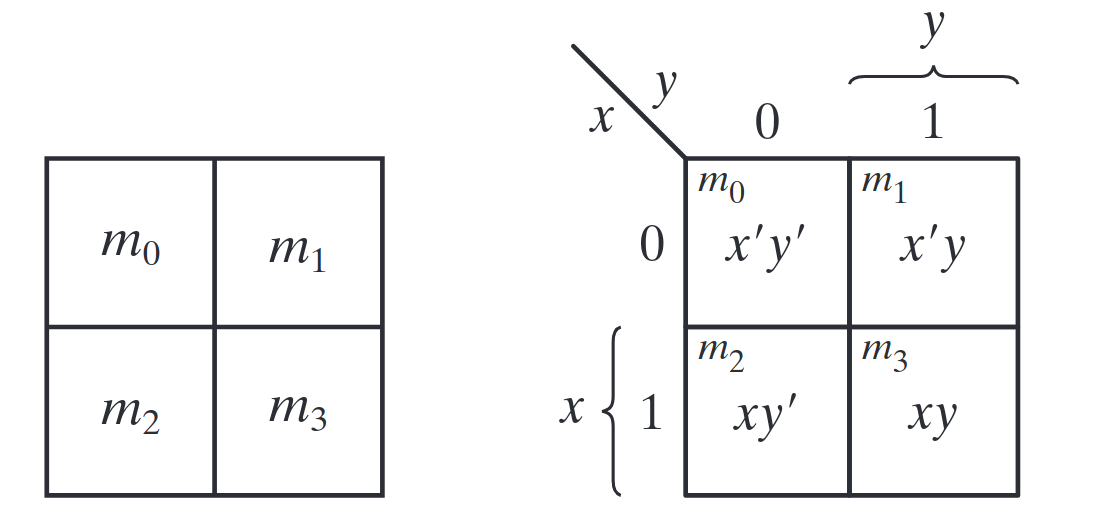
\includegraphics[width=0.5\textwidth]{figs/2var.png}fi
\caption{2-variable K-map structure and minimization example}
\label{fig:2var}
\end{figure}

\section{2-Variable K-Maps}
\subsection{Structure and Minimization}
\begin{itemize}
\item 4 cells representing minterms m0-m3
\item Horizontal axis: variable x
\item Vertical axis: variable y
\end{itemize}

\textbf{Example Simplification}:
\begin{equation}
F(x,y) = \sum(0,1,3) \Rightarrow x' + y
\end{equation}

\begin{figure}[htbp]
\centering
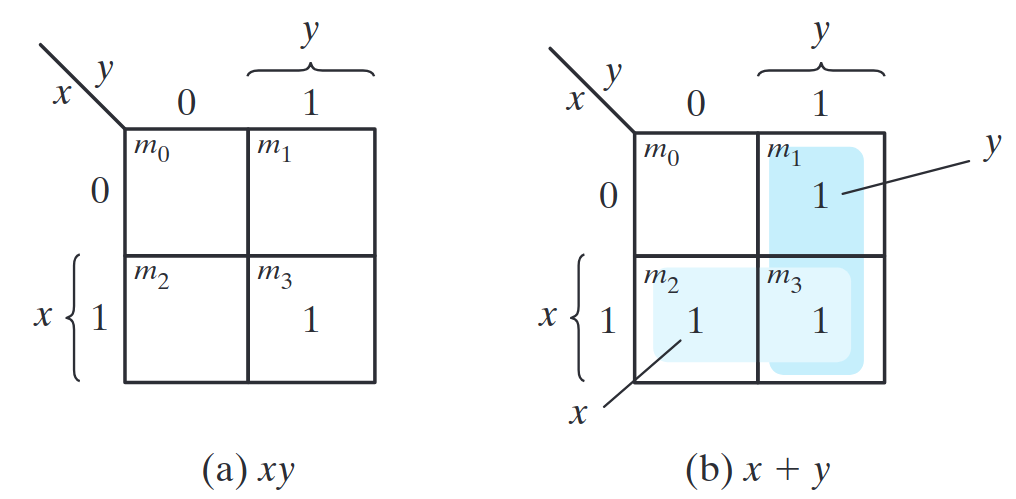
\includegraphics[width=0.4\textwidth]{figs/2ex.png}
\caption{2-variable K-map example minimization}
\label{fig:2ex}
\end{figure}

\section{3-Variable K-Maps}
\subsection{Layout and Adjacency Rules}
\begin{itemize}
\item 8 cells arranged in 2x4 grid
\item Variables typically ordered as x,y,z
\item Wrapping adjacency between left-right columns
\end{itemize}

\begin{figure}[htbp]
\centering
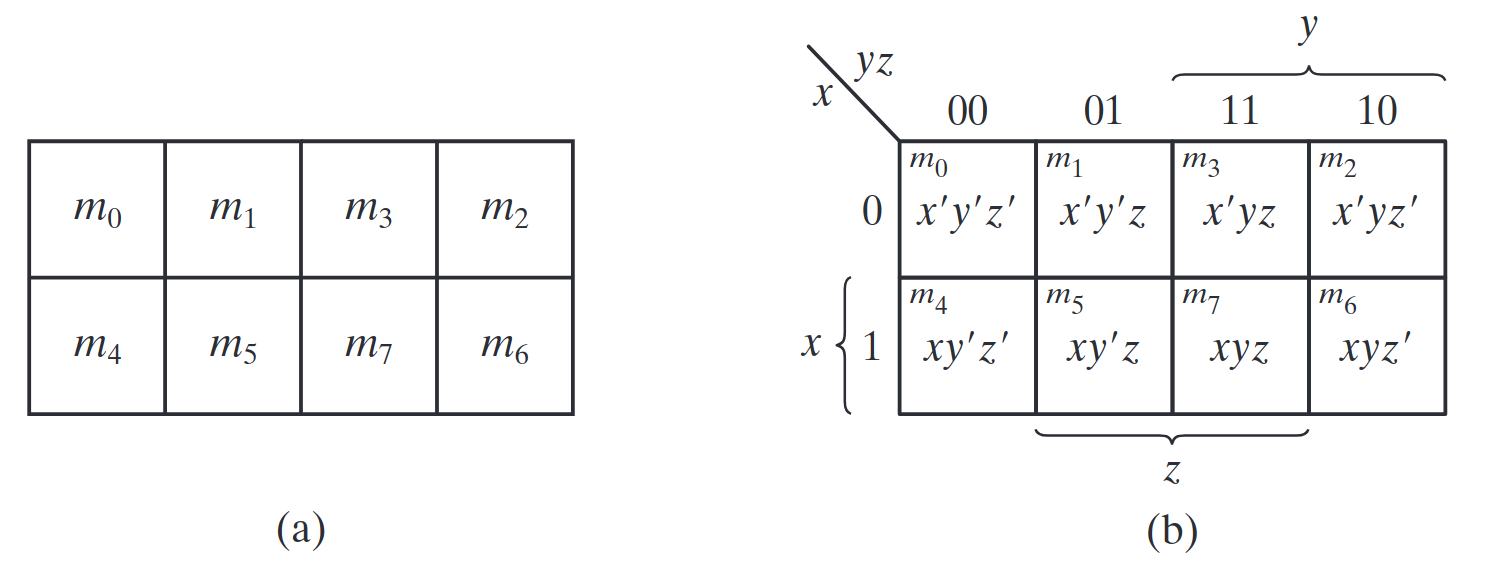
\includegraphics[width=0.6\textwidth]{figs/3var.png}
\caption{3-variable K-map structure}
\label{fig:3var}
\end{figure}

\subsection{Minimization Examples}
\begin{enumerate}
\item $F = \sum(2,3,4,5) \Rightarrow x'y + xy'$
\item $F = \sum(3,4,6,7) \Rightarrow yz + xz'$
\item $F = \sum(0,2,4,5,6) \Rightarrow z' + xy'$
\end{enumerate}

\section{4-Variable K-Maps}
\subsection{Structure and Simplification}
\begin{itemize}
\item 16 cells arranged in 4x4 grid
\item Both horizontal and vertical wrapping
\item Typical variable order: w,x,y,z
\end{itemize}

\begin{figure}[htbp]
\centering
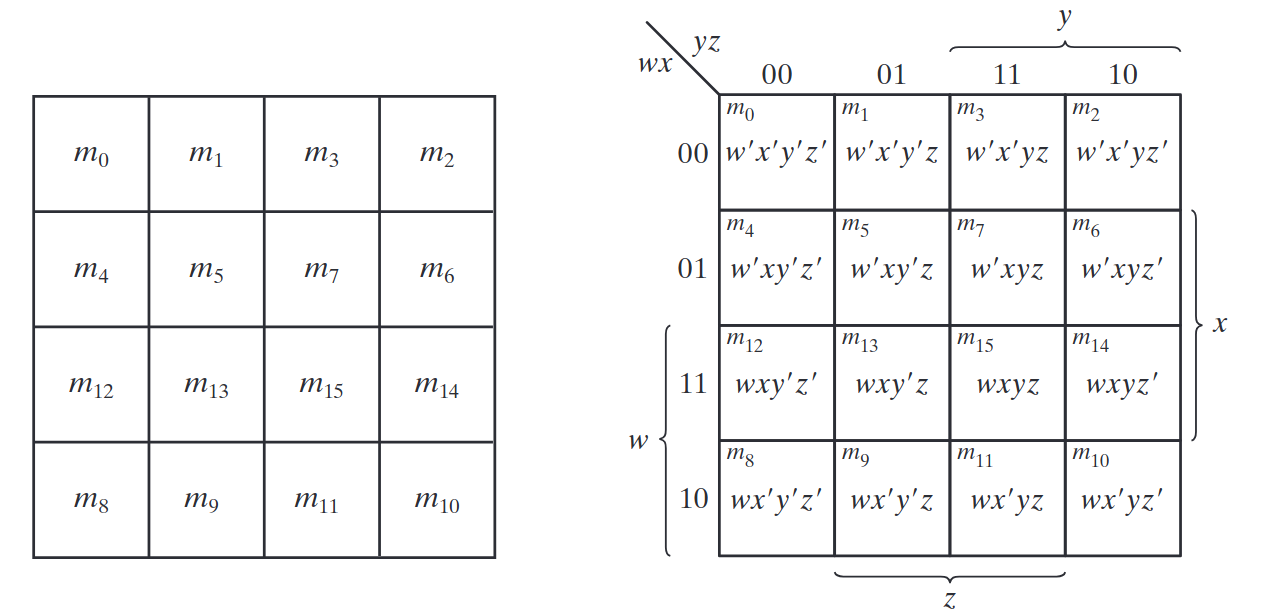
\includegraphics[width=0.7\textwidth]{figs/4var.png}
\caption{4-variable K-map layout}
\label{fig:4var}
\end{figure}

\textbf{Example Minimization}:
\begin{equation}
F = \sum(0,1,2,4,5,6,8,9,12,13,14) \Rightarrow y' + w'z' + xz'
\end{equation}

\section{Prime Implicants}
\subsection{Key Concepts}
\begin{itemize}
\item \textbf{Prime Implicant}: Maximal group of adjacent 1s
\item \textbf{Essential PI}: Contains at least one unique minterm
\item Non-essential PIs: Can be replaced by alternative combinations
\end{itemize}

\begin{figure}[htbp]
\centering
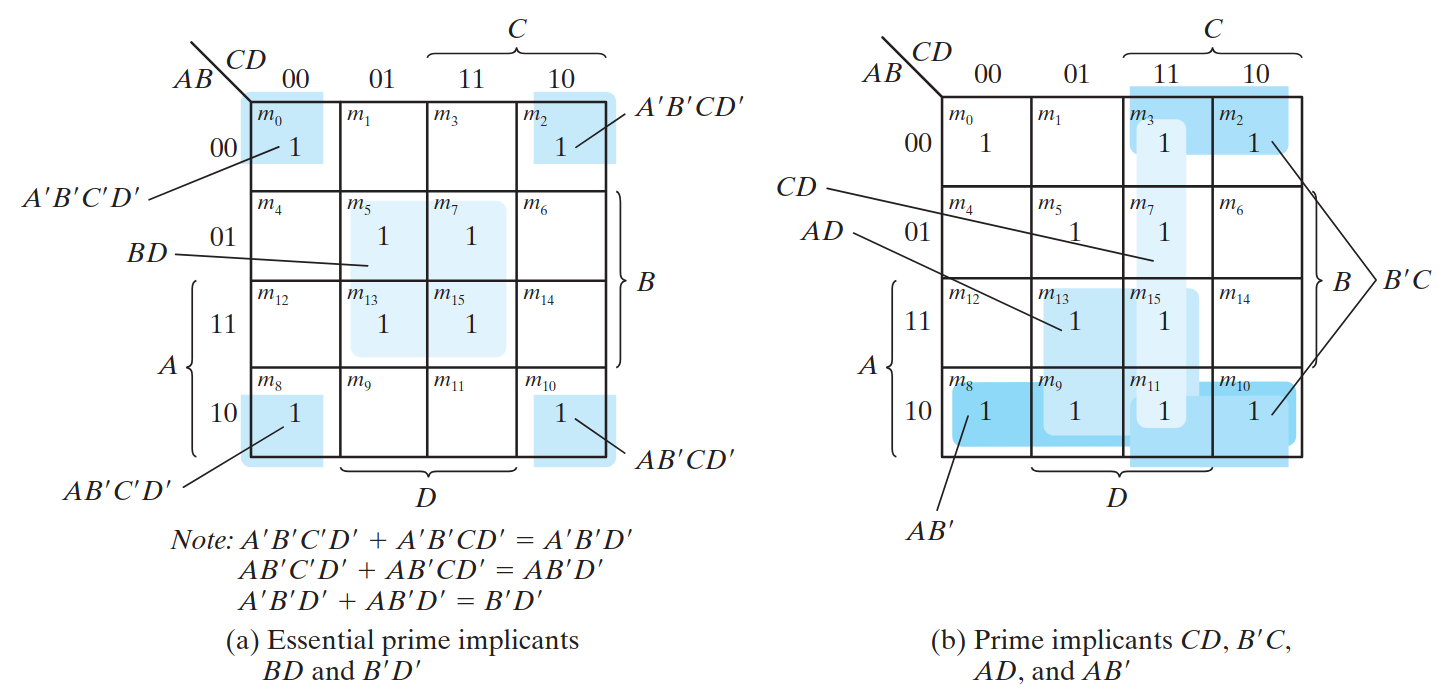
\includegraphics[width=0.6\textwidth]{figs/pr.png}
\caption{Prime implicant selection example with multiple solutions}
\label{fig:prime}
\end{figure}

\section{Product-of-Sums Simplification}
\subsection{SOP vs POS Implementation}
\begin{table}[htbp]
\centering
\begin{tabular}{p{0.45\textwidth}p{0.45\textwidth}}
\toprule
\textbf{Sum-of-Products (SOP)} & \textbf{Product-of-Sums (POS)} \\
\midrule
AND-OR structure & OR-AND structure \\
Minimize 1s in K-map & Minimize 0s in K-map \\
Direct implementation & Complemented implementation \\
\bottomrule
\end{tabular}
\caption{Comparison of SOP and POS implementations}
\end{table}

\section{Don't Care Conditions}
\subsection{Handling Incomplete Functions}
\begin{itemize}
\item X-marked cells represent don't care conditions
\item Can be treated as 0 or 1 for better minimization
\item Particularly useful in BCD and error-checking circuits
\end{itemize}

\begin{figure}[htbp]
\centering
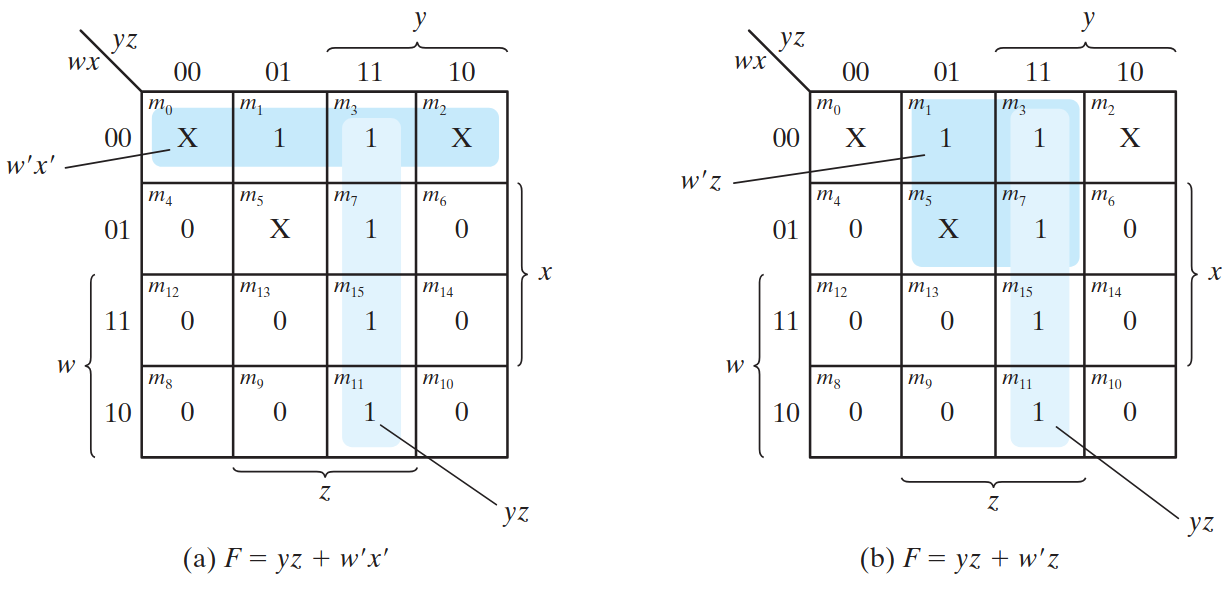
\includegraphics[width=0.8\textwidth]{figs/don.png}
\caption{Don't care condition utilization example}
\label{fig:dontcare}
\end{figure}

\section{Conclusion}
Key takeaways from gate-level minimization:
\begin{itemize}
\item K-maps provide systematic visual simplification
\item Proper identification of prime implicants is crucial
\item Don't care conditions enable more efficient designs
\item Fundamental for both manual design and automated tools
\end{itemize}

\end{document}
